\def\pgfsysdriver{pgfsys-dvipdfm.def}
\documentclass[aspectratio=169]{beamer}
\usepackage{fontspec}
\setmainfont[Mapping=tex-text]{Arial}
\setsansfont[Mapping=tex-text]{Arial}
\setmonofont[Mapping=tex-text]{Arial}
\usepackage[russian]{babel}
\usetheme{default}
%\setbeameroption{show notes}
\usepackage{listings}
\usepackage{hyperref}
\usepackage{caption}
\usepackage{subcaption}
\usepackage{tabularx}
\usepackage{advdate}
\usepackage{pgfpages}
\usepackage{pifont}
%\renewcommand\tabularxcolumn[1]{m{#1}}   

\usepackage{adjustbox}
\usepackage{tabularx}

\usepackage{tikz}
\usetikzlibrary{automata,positioning,arrows.meta,calc,shapes.geometric}
\tikzset{>={Stealth[width=3mm,length=3mm]}}

%-------------------------------------------------------------------------------
\setbeamertemplate{navigation symbols}{}
\setbeamertemplate{itemize subitem}{\ding{226}}
\setbeameroption{hide notes} % Only slides
%\setbeameroption{show only notes} % Only notes
% \setbeameroption{show notes on second screen=right} % Both
\setbeamertemplate{note page}{\pagecolor{yellow!5}\vfill\insertnote\vfill}
\setbeamertemplate{headline}{%
\leavevmode%
    \hbox{%
        \begin{beamercolorbox}[wd=\paperwidth,ht=2.25ex,dp=1ex,center]{section in head/foot}%
            \usebeamerfont{section in head/foot}\insertsectionhead
        \end{beamercolorbox}%
    }
}
\makeatletter
\setbeamertemplate{footline}
{
    \leavevmode%
    \hbox{%
        \begin{beamercolorbox}[wd=.333333\paperwidth,ht=2.25ex,dp=1ex,center]{date in head/foot}%
            \usebeamerfont{author in head/foot}\insertshortauthor
        \end{beamercolorbox}%
        \begin{beamercolorbox}[wd=.333333\paperwidth,ht=2.25ex,dp=1ex,center]{date in head/foot}%
            \usebeamerfont{title in head/foot}\insertshorttitle
        \end{beamercolorbox}%
        \begin{beamercolorbox}[wd=.333333\paperwidth,ht=2.25ex,dp=1ex,right]{date in head/foot}%
            \usebeamerfont{date in head/foot}\insertshortdate{}\hspace*{2em}
            \insertframenumber{} / \inserttotalframenumber\hspace*{2ex} 
        \end{beamercolorbox}}%
        \vskip0pt%
    }
\makeatother

%-------------------------------------------------------------------------------
\title[]{Универсальный механизм первичного поиска повторов в тексте для пакета Duplicate Finder}
\author[Глазырин Антон]{Глазырин Антон Георгиевич, 21.М07-мм\\[1ex] 
 {\small Научный руководитель: доц. каф. СП, к.ф-м.н. Д.\,В. Луцив\\}}
\institute[]{СПбГУ}
\date{\SetDate[18/05/2023]\today}

\begin{document}
	
%==============================================================================

\begin{frame}
\titlepage
\end{frame}

%==============================================================================

\begin{frame}\frametitle{Мотивация}
\begin{itemize}
	\item E. Juergens, J. Porubän: $\approx$10\% документации --- дублированные фрагменты
	\item Негативное влияние повторов:
	\begin{itemize}
		\item Раздувание объема
		\item Усложнение модификации
	\end{itemize}
	\item Управление повторами --- улучшение документации
\end{itemize}
\end{frame}

%==============================================================================

\begin{frame}\frametitle{Мотивация: Duplicate Finder}
	\begin{figure}
		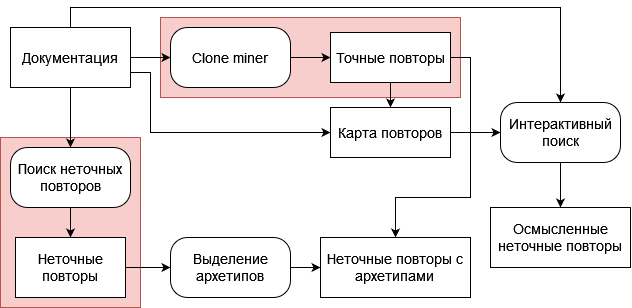
\includegraphics[scale=0.45]{../diploma/pictures/DuplicateFinder.png}
	\end{figure}
\end{frame}

%==============================================================================

\begin{frame}\frametitle{Постановка задачи}
	Цель --- разработка унифицированной подсистемы поиска точных и неточных повторов для Duplicate Finder Toolkit.	
	
	\begin{itemize}
		\item Анализ предметной области
		\item Определение проблем поиска повторов в DuplicateFinder и требований к новому механизму
		\item Проектирование конвейера механизма поиска повторов
		\item Разработка алгоритмов точного и неточного поиска
		\item Реализация инструмента и его интеграция в DuplicateFinder
		\item Проведение тестирования разработанного инструмента
	\end{itemize}
\end{frame}

%==============================================================================

\begin{frame}\frametitle{Существующие решения}
	\begin{itemize}
		\item Поиск клонов в ПО:
		\begin{itemize}
			\item CloneMiner
			\item CCFinder
			\item Klocwork inSight
			\item cpdetector
		\end{itemize}
		\item Сравнение текстовых документов:
		\begin{itemize}
			\item Align
			\item TxtAlign
		\end{itemize} 
		\item Поиск по образцу: 
		\begin{itemize}
			\item Duplicate Defect Detection
			\item Apache Lucene
			\item FactorLCS
		\end{itemize}
	\end{itemize}
\end{frame}

%===============================================================================

\begin{frame}\frametitle{Определение требований}
	\begin{enumerate}
		\item Реализация на языке Python.
		\item Поиск точных и неточных повторов.
		\item Универсальность процесса поиска.
		\item Наличие API и CLI.
		\item Возможности конфигурации.
	\end{enumerate}
\end{frame}

%===============================================================================

\begin{frame}\frametitle{Конвейер поиска повторов}
	\begin{figure}
		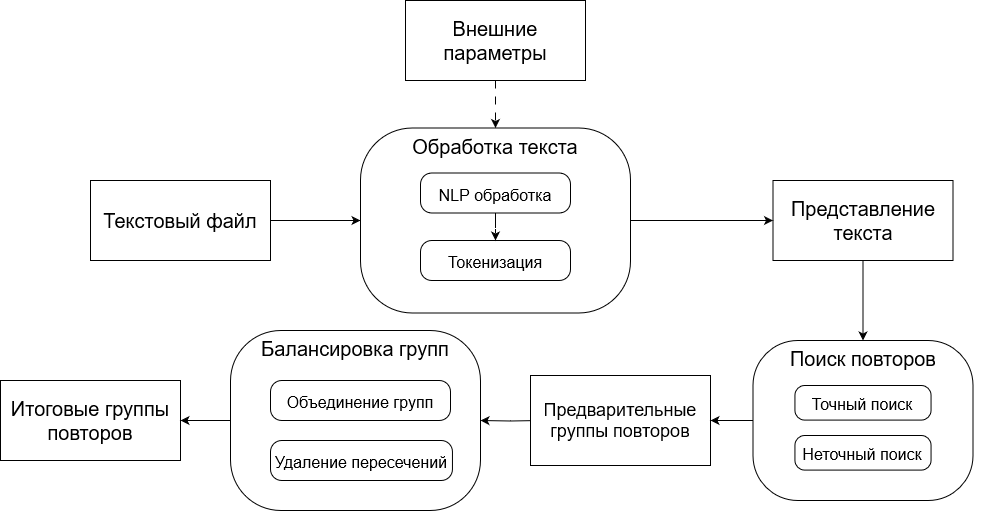
\includegraphics[scale=0.36]{../diploma/pictures/Flowchart.png}
	\end{figure}
\end{frame}


%===============================================================================

\begin{frame}\frametitle{Предобработка текста}
Методы NLP:
\begin{itemize}
	\item Фильтрация спецсимволов
	\item Удаление стоп слов
	\item Лемматизация
	\item Стемминг
\end{itemize}
\end{frame}


%===============================================================================

\begin{frame}\frametitle{Поиск точных повторов}

\begin{figure}
	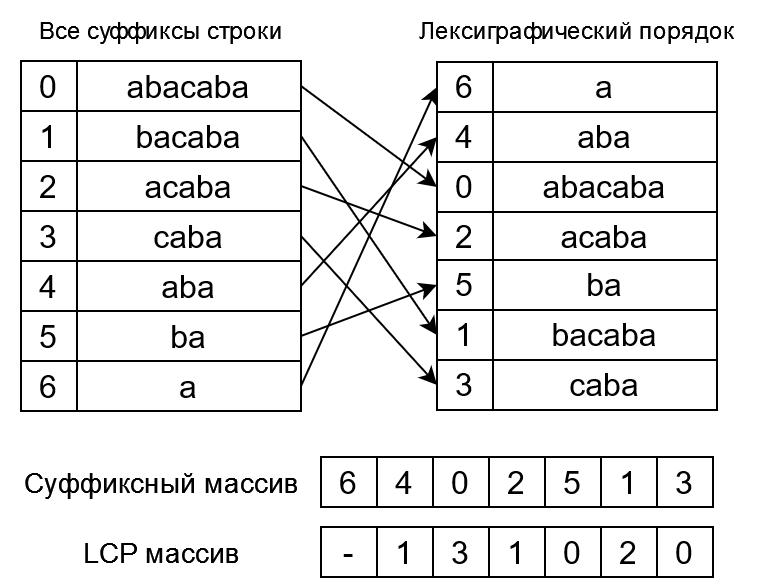
\includegraphics[scale=0.3]{../diploma/pictures/SA-LCP.png}
\end{figure}

\end{frame}

%===============================================================================

\begin{frame}\frametitle{Поиск неточных повторов I}
	Расстояние Левенштейна:
	
	\begin{figure}
		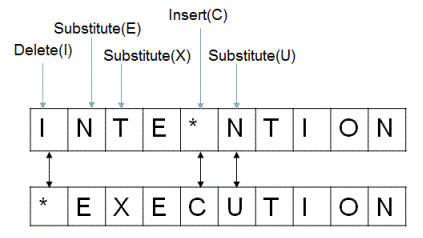
\includegraphics[scale=0.45]{../diploma/pictures/edit_dist.png}
	\end{figure}

\end{frame}

%===============================================================================

\begin{frame}\frametitle{Поиск неточных повторов I}
	SimHash:
	
	\begin{figure}
		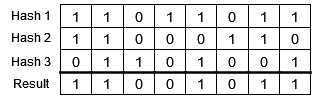
\includegraphics[scale=0.7]{../diploma/pictures/Hash.png}
	\end{figure}
\end{frame}

%===============================================================================

\begin{frame}\frametitle{Поиск неточных повторов II}
	Множества N-грамм:
	\begin{figure}
		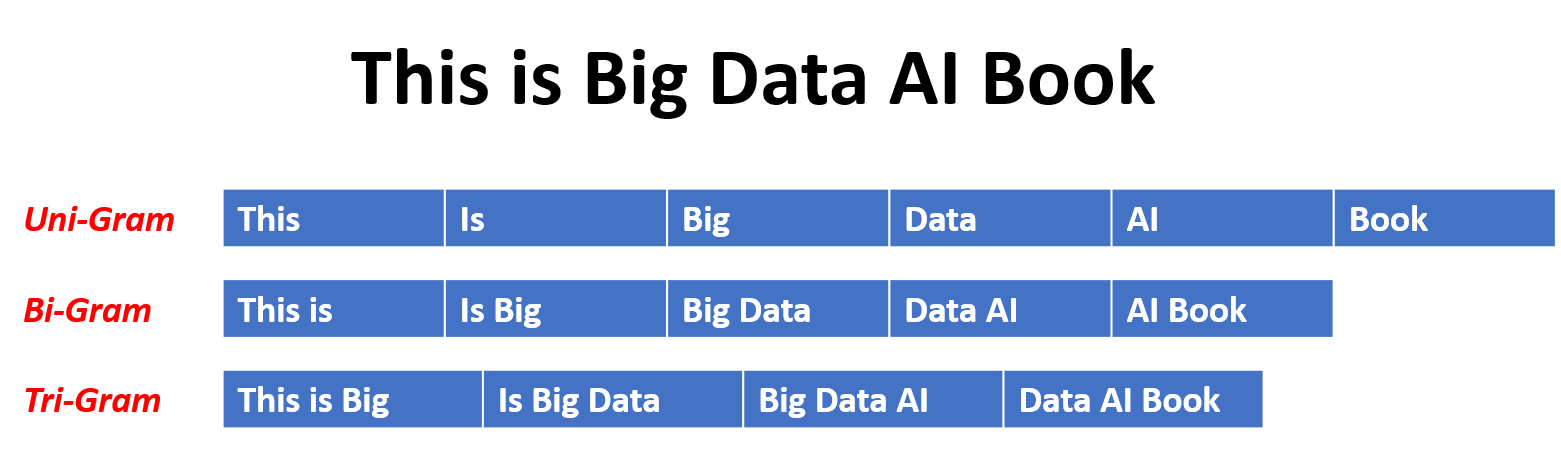
\includegraphics[scale=0.3]{../diploma/pictures/ngram.png}
	\end{figure}
\end{frame}

%===============================================================================

\begin{frame}\frametitle{Балансировка групп повторов}
	\begin{itemize}
		\item Фильтрация незначимых групп
		\item Слияние фрагментов
	\end{itemize}

	\begin{figure}
		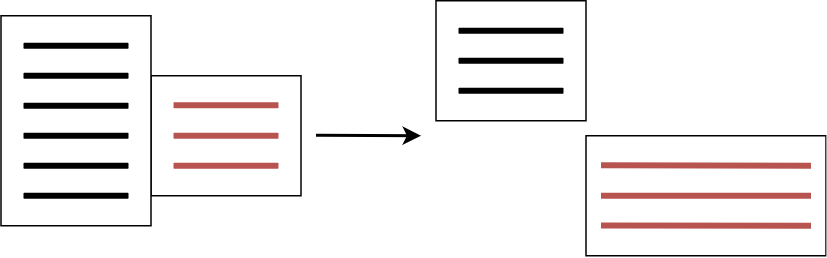
\includegraphics[scale=0.3]{../diploma/pictures/Balance3.png}
	\end{figure}
\end{frame}

%===============================================================================

\begin{frame}\frametitle{Архитектура}
	\begin{figure}
		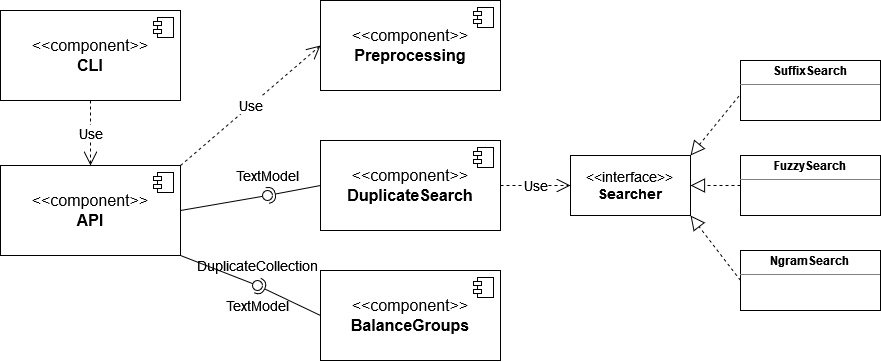
\includegraphics[scale=0.45]{../diploma/pictures/Architecture.png}
	\end{figure}
\end{frame}

%===============================================================================

\begin{frame}\frametitle{Тестирование: точный поиск}
	\begin{figure}[h!]
		\centering
		\begin{minipage}{0.9\textwidth}
\begin{adjustbox}{center}
\begin{tabular}{|l||c|c|c|c|}
	\hline
	& GIMP & PostgreSQL & Subversion & Zend Framework \\
	\hline
	\hline
	Токены & 132554 & 72728 & 110270 & 164035 \\
	\hline
	Группы повторов & 400 & 289 & 218  & 557 \\
	\hline
	Средний размер группы & 2.57 & 2.30 & 2.17 & 2.44 \\
	\hline
	Средняя длина повтора & 14.59 & 16.31 & 17.27 & 16.58 \\
	\hline
	Покрытие документа & ~11\% & ~14\% & ~7\% & ~13\% \\
	\hline
	
\end{tabular}
\end{adjustbox}
\end{minipage}
	\end{figure}
\end{frame}
%===============================================================================

\begin{frame}\frametitle{Тестирование: неточный поиск}
	
	\begin{figure}[h!]
		\centering
		\begin{minipage}{0.9\textwidth}
\begin{adjustbox}{center}
\begin{tabular}{|l||m{0.15\textwidth}|m{0.15\textwidth}|m{0.15\textwidth}|m{0.2\textwidth}|}
	\hline
	Документ & Группы повторов & Средний размер группы & Средняя длина повтора & Покрытие документа \\
	\hline
	\hline
	GIMP Manual & 574 & 2,65 & 13,64 & 15\% \\
	\hline
	PostgreSQL Manual & 464 & 2,66 & 17,17 & 25\% \\
	\hline
	Subversion book & 282 & 2,27 & 18,93 & 10\% \\
	\hline
	Zend Framework guide & 522 & 2,32 & 22,96 & 16\% \\
	\hline
	Blender Manual & 1393 & 2,48 & 14,22 & 16\% \\
	\hline
	Python Requests & 23 & 2,26 & 20,16 & 28\% \\
	\hline
\end{tabular}
\end{adjustbox}
\end{minipage}
	\end{figure}
	
\end{frame}

%===============================================================================

\begin{frame}\frametitle{Заключение}
	
\begin{enumerate}
	\item Проанализированы основные подходы и средства, которые используются в существующих инструментах для поиска повторов.
	\item Выявлены требования к новому механизму поиска.
	\item Спроектирован конвейер для механизма поиска: предобработка текста, применение алгоритмов поиска повторов, балансировка групп повторов.
	\item Разработаны алгоритмы для точного и неточного поиска повторов на основе использованных в Duplicate Finder инструментов.
	\item Выполнена реализация инструмента на языке Python с использованием пакета NLTK для предобработки текста, исходный код выложен на GitHub; проведена интеграция с Duplicate Finder.
	\item Проведено тестирование инструмента на корпусе документов, по результатам работы собрана статистика и проведен ее анализ.
\end{enumerate}

\end{frame}

%===============================================================================

\end{document}